\section{Fanny Shafira Damayanti (1174069)}
\subsection{Teori}
\begin{enumerate}
\item Definisi Kecerdasan buatan\\ 
Kecerdasan buatan atau Artificial intelligence merupakan kecerdasan yang ditambahkkan kedalam suatu system yang diatur secara ilmiah. Kecerdasan buatan dibuat untuk menggantikan pekerjaan yang dilakukan oleh manusia menjadi dikerjakan oleh sistem.

\item Sejarah Kecerdasan Buatan
\begin{itemize}
\item Abad 17, Rene Descartes berkata bahwa tubuh hewan adalah sekumpulan mesin yang rumit.
\item 1642, Blaise Pascal menciptakan mesin penghitung digital mekanis pertama.
\item Abad 19, Charles Babbage dan Ada Lovelace bekerja di program penghitung mekanis.
\item 1950, John McCarthy membuat istilah “Kecerdasan Buatan”.
\item 1960-1970, Joel Moses membuat program yang pertama kali sukses dalam bidang matematika.
\item 1980, jaringan saraf digunakan secara meluas dengan algoritme perambatan balik.
\item 2004, DARPA membuat kendaraan yang bisa dijalankan sendiri tanpa manusia.
\end{itemize}

\item Perkembangan kecerdasan buatan
\begin{itemize}
\item Masa persiapan (1943-1946)
Warren McCulloch dan Walter Pitt mengemukakan tiga hal : pengetahuan fisiologi dasar dan fungsi sel syaraf dalam otak, analisa formal tentang logika proposisi, dan teori komputasi Turing.

Pada tahun 1950, Nobert Wiener membuat penelitian mengenai prinsip-prinsip teori feedback.

Pada tahun 1956, John McCarthy meyakinkan Minsky, Claude Shannon dan Nathaniel Rochester untuk membantunya melakukan penelitian dalam bidan Otomata, Jaringan Syaraf dan pembelajaran intelijensia. 

\item Awal perkembangan (1952-1969)
Pada tahun 1958, McCarthy di MIT AI Lab Memo No.1 mendefinisikan bahasa pemrograman tingkat tinggi yaitu LISP,

Pada tahun 1959, Nathaniel Rochester dari IBM dan mahasiswa-mahasiswanya mengeluarkan program kecerdasan buatan yaitu Geometry Theorm Prover.

Pada tahun 1963, program yang dibuat James Slagle mampu menyelesaikan masalah integral tertutup untuk mata kuliah Kalkulus.
Pada tahun 1986, program analogi buatan Tom Evan menyelesaikan masalah analogi geometris yang ada pada tes IQ.

\item Perkembangan Kecerdasan Buatan Melambat (1969-1979)
Bruce Buchanan dan Joshua Lederberg yang membuat program untuk memecahkan masalah struktur molekul dari informasi yang didapatkan dari spectrometer massa.

\item AI Menjadi sebuah industri
Industrialisasi kecerdasan buatan diawali dengan ditemukannya sistem pakar yang dinamakan R1 yang mampu mengkonfigurasi system-sistem computer baru. 

\item Kembalinya Jaringan Syaraf Tiruan (1986-sekarang)
Pada tahun 1985-an setidaknya empat kelompok riset menemukan kembali algoritma belajar propagasi balik (Black-Propagation Learning). Algoritma ini berhasil diimplementasikan ke dalam bidang ilmu computer dan psikologi.
\end{itemize}

\item Definisi Supervised Learning\\
Supervised Learning merupakan cabang dari Artificial Intelligence. supervised learning adalah suatu ilmu yang mempelajari perancangan dan pengembangan algoritma.

\item Klasifikasi Supervised Learning
\begin{itemize}
\item Logistic regression.
\item K-nearest neighbors.
\item Support vector machine (SVM)
\item Naive Bayes.
\item Decision tree classification.
\item Random forest classification.
\end{itemize}

\item Regresi dan Unsupervised Learning\\
Regresi merupakan sebuah metode analisis statistic yang digunkan untuk mengetahui pengaruh antara dua variable atau lebih.

Untuk mempelajari Unsupervised learning kita tidak perlu data training untuk melakukan prediksi maupun klasifikasi.

\item Dataset\\
Dataset merupakan objek yang mempresentasikan data dan relasinya pada memori.

\item Training Set\\
Training Set merupakan bagian dari dataset untuk membuat prediksi atau menjalankan fungsi dari sebuah algoritma Machine Learning.

\item Testing Set\\
Testing set digunakan untuk mengukur apakah classifier berhasil melakukan klasifikasi dengan benar.

\end{enumerate}

\subsection{Instalasi}
\begin{enumerate}
	\item Instalasi Library scikit dari anaconda, mencoba kompilasi dan uji coba ambil contoh kode dan lihat variabel explorer
	\hfill\break
	\begin{figure}[H]
		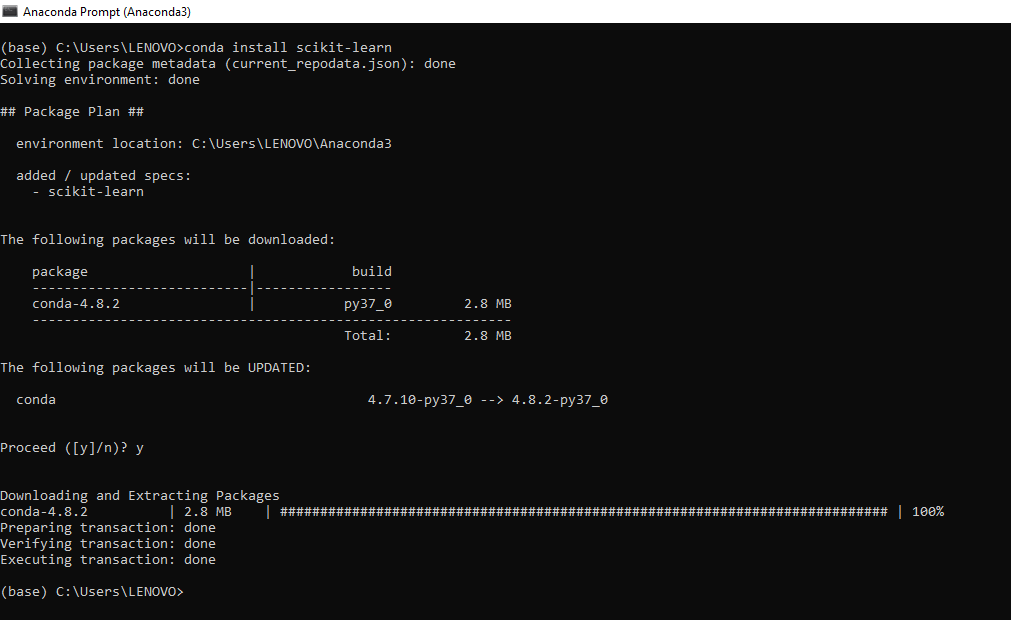
\includegraphics[width=4cm]{figures/1174069/1/1.png}
		\centering
		\caption{Instalasi Package Scikit Learn}
	\end{figure}
	\begin{figure}[H]
		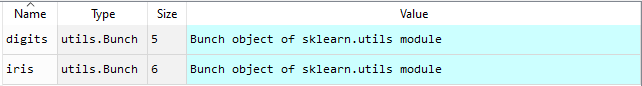
\includegraphics[width=4cm]{figures/1174069/1/2.png}
		\centering
		\caption{Isi Variabel Explorer}
	\end{figure}
	\item Mencoba Loading an example dataset, menjelaskan maksud dari tulisan tersebut dan mengartikan           		  per baris
	\hfill\break
	\lstinputlisting[firstline=7, lastline=11]{src/1174069/1/1174069.py}
	\item Mencoba Learning and predicting, menjelaskan maksud dari tulisan tersebut dan mengartikan per  			  baris
	\hfill\break
	\lstinputlisting[firstline=13, lastline=22]{src/1174069/1/1174069.py}
	\item  Mencoba Model persistence, menjelaskan maksud dari tulisan tersebut dan mengartikan per baris
	\hfill\break
	\lstinputlisting[firstline=25, lastline=34]{src/1174069/1/1174069.py}
	\item Mencoba Conventions, menjelaskan maksud dari tulisan tersebut dan mengartikan per baris
	\hfill\break
	\lstinputlisting[firstline=37, lastline=48]{src/1174069/1/1174069.py}
\end{enumerate}

\subsection{Penanganan Error}
\begin{enumerate}
	\item ScreenShoot Error
	\begin{figure}[H]
		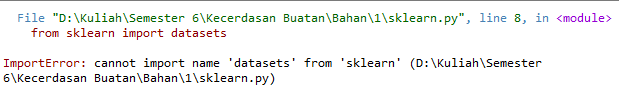
\includegraphics[width=4cm]{figures/1174069/1/error/1.png}
		\centering
		\caption{Import Error}
	\end{figure}

	\item Tuliskan Kode Error dan Jenis Error
	\begin{itemize}
		\item Import Error
	\end{itemize}
	\item Cara Penangan Error
	\begin{itemize}
		\item Import Error
		\hfill\break
		Dengan Menginstall Library Yang Tidak Ditemukan
	\end{itemize}
\end{enumerate}

\subsection{Bukti Tidak Plagiat}
\begin{figure}[H]
	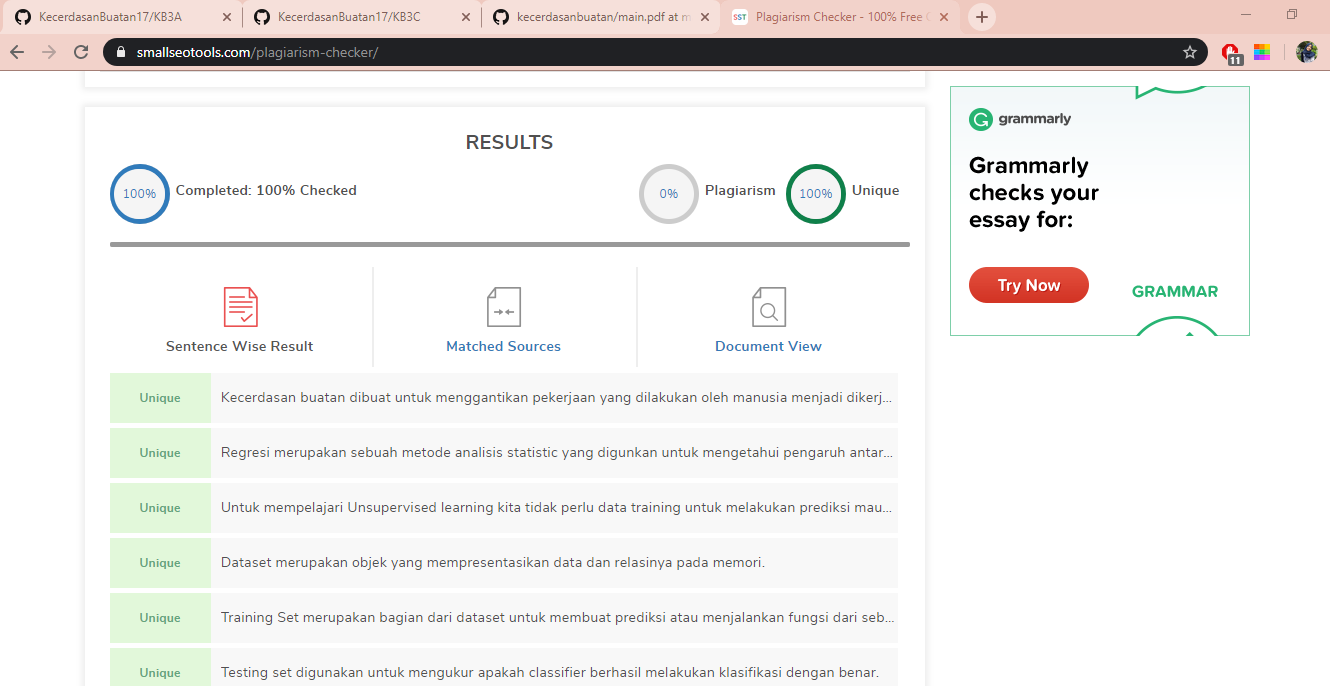
\includegraphics[width=4cm]{figures/1174069/1/plagiat/plagiat.png}
	\centering
	\caption{Bukti Tidak Melakukan Plagiat Chapter 1}
\end{figure}

\subsection{Link Youtube}

